%%
%%
%%
\subsubsection{\label{sec:streamsClassifiers}Embedding Classifiers in \streams}
From a high level viewpoint, an online classifier is able to
continuously learn on training data and give out predictions for
instances based on its current model/state. The following figure% \ref{fig:onlineLearning}
shows the division of this behavior into two parts:
\begin{figure}[h!]
  \centering
  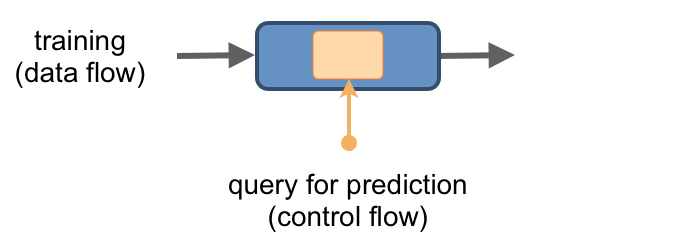
\includegraphics[scale=0.35]{graphics/online-learning.png}
%  \caption{\label{fig:onlineLearning}Learning on a stream and delivering predictions at any time.}
\end{figure}

\vspace{-2ex}
This abstract functionality provided by classifiers from the
perspective of the \streams framework encapsulates two functions:
\begin{enumerate}
\item {\bf Training:} Incorporate new data items into a prediction
  model.
\item {\bf Application:} Provide a prediction for a data item based on
  the current model.
\end{enumerate}
These two tasks are mapped onto two different aspects of the compute
graph that builds the basis for the streaming processes. The {\em
  training} is considered to be part of the general data flow,
i.e. data items are processed by classifiers and will be used to
enhance the prediction model provided by the classifier.

The model {\em application}, i.e. the prediction based on the current
model of the classifier, is regarded as an {\em anytime service} that
is provided by the classifier. This service provides a {\ttfamily
  predict(Data)} function that is expected to return the prediction of
the classifier.

\subsubsection*{Providing Predictions at any time}
With the requirements for continuous data that we introduced in the
very beginning, the main concern is, that classifiers need to be able
to provide predictions at any time. With the {\em control flow} layer
provided by the notion of services, the \streams framework integrates
a tool for querying services from ``outside'', i.e. not using the data
flow.
\begin{figure}[b]
  \centering
  \begin{lstlisting}[language=Java]
     public interface Classifier extends Service {
         /**
          * This method returns a simple prediction based on the given
          * data item. The prediction is a general serializable value.
          */
         public Serializable predict( Data item );
     }
  \end{lstlisting}
  \caption{\label{fig:classifierService}The {\ttfamily Classifier}
    service interface that needs to be implemented by classifiers in
    the \streams framework. The return type of the {\ttfamily predict}
    method might be a number, e.g. for regression or a String, Integer
    or similar for a classification task.}
\end{figure}
Such services are registered within the container and can be
queried from other containers or being exported (e.g. via Java RMI).


\subsubsection{\label{sec:addPrediction}Using the Classifier service}
The example in Figure \ref{fig:exampleWithKeys} shows the use of a
classifier that is added to the data flow for constant training. The
referenced {\ttfamily NaiveBayes} class implements the {\ttfamily
  Processor} interface and additional supports the {\ttfamily
  Classifier} interfaces shown in \ref{fig:classifierService}. The
{\ttfamily id} of the classifier (processor) specifies the name under
which that classifier is registered within the naming service of the
container.

After initialization time, the classifier is registered and can be
queried using Java RMI or by other processors from within the
container (or connected containers). This is illustrated in the
following abstraction (Figure \ref{fig:serviceProcessors}): The 
process within that graph contains a processor that provides a
service (marked in orange) and another process that references
that services, i.e.~plays the role of a {\em service consumer}.

\begin{figure}[h!]
  \centering
  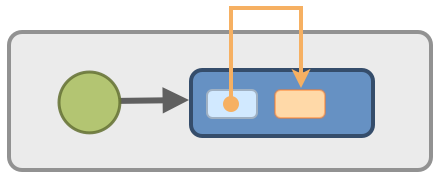
\includegraphics[scale=0.3]{graphics/add-prediction.png}
  \caption{\label{fig:serviceProcessors}A processor using a processor
    that provides a services (e.g. Classification).}
\end{figure}

\subsubsection*{Adding Predictions}
One of the processors that can be used to add predictions based on
classifier services is the {\ttfamily AddPrediction} class. This
processor references a classifier service by its {\ttfamily id} and
calls the {\ttfamily predict(Data)} method for every item it
processes.

The prediction of the classifier is then added to the data item with
an attribute key {\ttfamily @prediction:} followed with the {\ttfamily
  id} of the service. An example is given in the XML snippet shown in
Figure \ref{fig:applyPrediction}. The {\ttfamily AddPrediction} element
will use the classifier for prediction and then add the prediction as
a special attribute with key {\ttfamily @prediction:NB} to the data item.
Since special attributes are to be discarded by the learning algorithms
by convention, it will not influence the training.
\begin{figure}[h!]
  \centering
  \begin{lstlisting}[language=XML]
     ...
     <process input="golf">
         <!-- pre-processing left out for brevity    -->

         <!-- apply a prediction to each data item based
              on the specified classifier               -->
         <stream.learner.AddPrediction classifier="NB" />

         <!-- consume the next data item and use it for
              learning.                                -->
         <stream.classifier.NaiveBayes id="NB" />
     </process>
  \end{lstlisting}
  \caption{\label{fig:applyPrediction}First predict, then learn on a data item.}
\end{figure}
